\documentclass{beamer}

\usepackage{../../latex_style/beamerthemeExecushares}
\usepackage{../../latex_style/notations}

\title{Session 1: Vector spaces}
\subtitle{Optimization and Computational Linear Algebra for Data Science}
\author{Léo Miolane}
\date{}

\setcounter{showSlideNumbers}{1}

\begin{document}
\setcounter{showProgressBar}{0}
\setcounter{showSlideNumbers}{0}

\frame{\titlepage}

\begin{frame}
	\frametitle{Contents}
	\begin{enumerate}
		\item Subspaces
		\item Linear dependency
		\item Properties of the dimension
		\item Coordinates
		\item Why do we care about all these things ? \below{Application to data science: image compression}
	\end{enumerate}
\end{frame}


\setcounter{framenumber}{0}
\setcounter{showSlideNumbers}{1}

\section{Logistics}

\begin{frame}[t]{The teaching team}

	\begin{itemize}
		\item \textbf{Lecturer}: \quad Léo Miolane \  -- \ \emph{lm4271\@nyu.edu}
			\below{\href{https://leomiolane.github.io/linalg-for-ds.html}{\texttt{leomiolane.github.io/linalg-for-ds.html}}}
\vspace{0.3cm}
		\item \textbf{Course assistant}: \quad Chen Li
			\vspace{0.3cm}
			\pause
		\item \textbf{Sections leaders}:
			\vspace{0.2cm}
			\begin{columns}
				\begin{column}{0.3\textwidth}
					\begin{center}
						Alex
						\\
						\vspace*{0.2cm}
						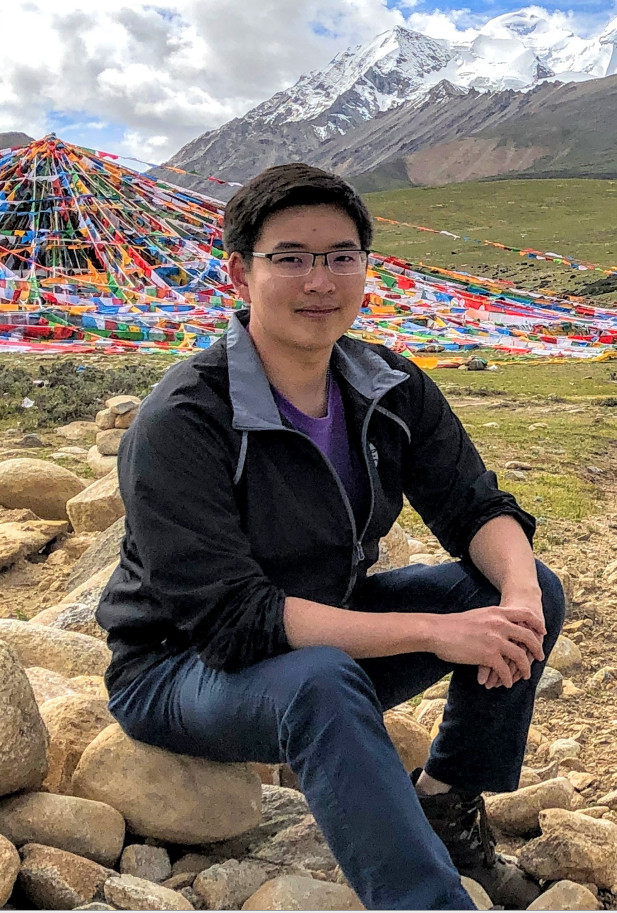
\includegraphics[height=2.5cm]{./alex.jpeg}
					\end{center}
				\end{column}
				\begin{column}{0.3\textwidth}
					\begin{center}
						Irina
						\\
						\vspace*{0.2cm}
						
\includegraphics[height=2.5cm]{./irina.jpeg}
					\end{center}
				\end{column}
				\begin{column}{0.3\textwidth}
					\begin{center}
						Carles
						\\
						\vspace*{0.2cm}
						
\includegraphics[height=2.5cm]{./carles.jpeg}
					\end{center}
				\end{column}
			\end{columns}
	\end{itemize}

\end{frame}

\begin{frame}[t]{Course components}
	Three main components:
	\begin{enumerate}
		\item Videos \below{2-3 short videos to watch \textbf{before} each lecture}
		\item Lectures \below{Deepens the concepts introduced in the videos}
		\item Recitations \below{Practice!}
	\end{enumerate}

	\vspace{0.5cm}
	\pause
	\textbf{Grades}:
	\begin{enumerate}
		\item Weekly quizzes (5\%)
		\item Weekly homeworks (40\%)
		\item Exams: Midterm (20\%) + Final (35\%)
	\end{enumerate}

\end{frame}
\begin{frame}{Weekly timeline}
	\begin{center}
		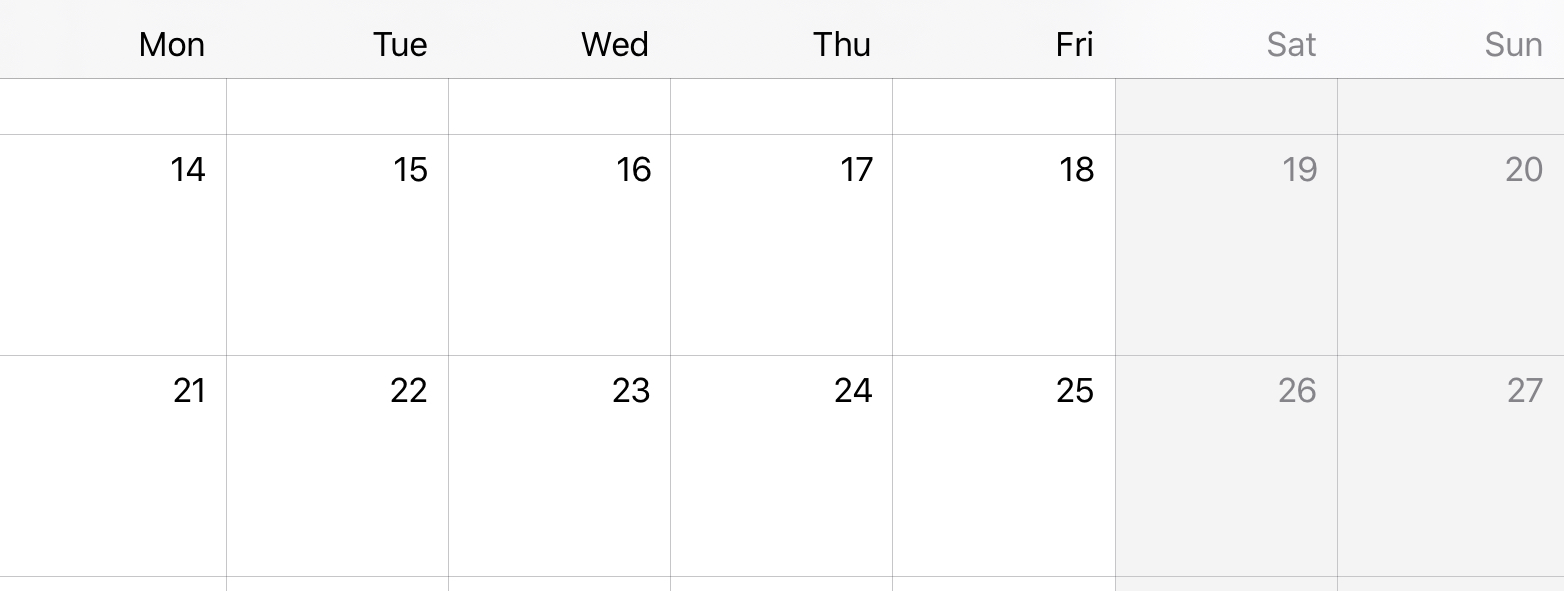
\includegraphics[width=\textwidth]{./timetable.jpg}
	\end{center}
\end{frame}

\begin{frame}{Grading}
	\begin{itemize}
		\item Quizzes have to be answered on \textbf{WebAssign}.
		\item Homeworks questions are available on the \textbf{course's webpage} and have to be submitted on \textbf{WebAssign}.
			\pause
		\item I encourage you to type your homeworks using \texttt{LaTeX}.
			\below{Help and template available on the course's webpage.}
		\item Otherwise, you can scan (using dedicated app) your handwritten work.
			{\bf It has to be legible!!!}
			\pause
		\item Midterm ($\sim$ mid-October) and Final will be <<take-home exams>>.
		\item Limited time: after downloading the Midterm/Final questions, you will have to upload your work within few hours.
	\end{itemize}
\end{frame}

\section{Questions ?}
\begin{frame}[t]{Questions ?}
	\pause
\end{frame}

\section{Subspaces}
\begin{frame}{What are the subspaces of $\R^2$ ?}
\end{frame}

\begin{frame}[t]{The span is always a subspace}
	\begin{block}{\bf Proposition}
		Let $x_1, \dots, x_k \in V$. Then, $\Span(x_1, \dots, x_k)$ is a subspace of $V$.
	\end{block}
\end{frame}

\section{Linear dependency}
\begin{frame}[t]{A useful lemma}
	\vspace{-0.4cm}
	\begin{block}{\bf Lemma}
		Let $v_1, \dots, v_n \in V$
		and let $x_1, \dots, x_k \in \Span(v_1, \dots, v_n)$.
		\\
		Then, if $k > n$,
		$x_1, \dots, x_k$ are linearly dependent.
	\end{block}
	\textbf{Abuse of language:} Instead of saying <<$x_1, \dots, x_k$ are linearly dependent>>, we should have said <<the family $(x_1, \dots, x_k)$ is linearly dependent>>.
\end{frame}

\section{Basis, dimension}
\begin{frame}[t]{The dimension is well defined!}
	\begin{block}{\bf Theorem}
		If $V$ admits a basis $(v_1, \dots, v_n)$, then every basis of $V$ has also $n$ vectors. We say that $V$ has dimension $n$ and write $\dim(V) = n$.
	\end{block}
	\begin{proof}
		\vspace{3cm}
		\vfill
	\end{proof}
\end{frame}
\begin{frame}[t]{Properties of the dimension}
	\vspace{-0.3cm}
	\begin{block}{\bf Proposition}
		Let $V$ be a vector space that has dimension $\dim(V) = n$. Then
		\begin{itemize}
			\item Any family of vectors of $V$ that are linearly independent contains at most $n$ vectors.
				\below{i.e.\ if $x_1, \dots, x_k \in V$ are linearly independent, then $k \leq n$.}
			\item Any family of vectors of $V$ that spans $V$ contains at least $n$ vectors.
				\below{i.e.\ if $x_1, \dots, x_k \in V$ are such that $\Span(x_1, \dots, x_k) = V$, then $k \geq n$.}
		\end{itemize}
	\end{block}
	\begin{proof}
		\vspace{2cm}
		\vfill
	\end{proof}
	\pause
\end{frame}

\begin{frame}[t]{Properties of the dimension}
	\vspace{-0.3cm}
	\begin{block}{\bf Proposition}
		Let $V$ be a vector space of dimension $n$ and let $x_1, \dots, x_n \in V$.
		\begin{enumerate}
			\item If $x_1, \dots, x_n$ are linearly independent, then $(x_1, \dots, x_n)$ is a basis of $V$.
			\item If $\Span(x_1, \dots, x_n) = V$, then $(x_1, \dots, x_n)$ is a basis of $V$.
		\end{enumerate}
	\end{block}

	\vspace{0.5cm}

	Very useful to show that a family of vector forms a basis!

	\vspace{0.5cm}

	\begin{proof}
		\vfill
	\end{proof}
\end{frame}

\begin{frame}[t]{An inequality}
	\begin{block}{\bf Proposition}
		Let	$U$ and $V$ be two subspaces of $\R^n$. Assume that $U \subset V$. Then
		$$
		\dim(U) \leq \dim(V) \leq n.
		$$
		If \textbf{moreover} $\dim(U) = \dim(V)$, then $U = V$.
	\end{block}
\end{frame}

\begin{frame}[t]{A bit of vocabulary}
	\begin{block}{\bf Definition}
		Let $S$ be a subspace of $\R^n$.
		\begin{itemize}
			\item We call $S$ a \emph{line} if $\dim(S) = 1$.
			\item We call $S$ an \emph{hyperplane} if $\dim(S) = n-1$.
		\end{itemize}
	\end{block}
\end{frame}

\section{Coordinates}
\begin{frame}[t]{Coordinates of a vector in a basis}
	\vspace{-0.4cm}
	\begin{block}{\bf Definition}
		If $(v_1, \dots, v_n)$ is a basis of $V$, then for every $x \in V$ there exists a unique vector $(\alpha_1, \dots, \alpha_n) \in \R^n$ such that
		$$
		x = \alpha_1 v_1 + \dots + \alpha_n v_n.
		$$
		We say that $(\alpha_1, \dots, \alpha_n)$ are the coordinates of $x$ in the basis $(v_1, \dots, v_n)$.
	\end{block}
	\begin{proof}
		\vspace{2.5cm}
		\vfill
	\end{proof}
\end{frame}

\begin{frame}[t]{Exercise}
	\vspace{-0.8cm}
	\begin{exampleblock}{}
		\begin{enumerate}
			\item Show that the vectors $v_1 = (1,1)$ and $v_2=(1,-1)$ form a basis of $\R^2$.
			\item Express the coordinates of $u=(x,y)$ in the basis $(v_1,v_2)$ in terms of $x$ and $y$.
		\end{enumerate}
	\end{exampleblock}
	\pause
\end{frame}

\section{Why do we care about this ?}
\begin{frame}{Application to image compression}
	\begin{columns}
		\begin{column}{0.5\textwidth}
			\begin{itemize}
				\item Image = Grid of pixels
				\item Represented as a vector $v \in \R^n$, for some large $n$.
				\item One need to store $n$ numbers.
			\end{itemize}
		\end{column}
		\begin{column}{0.5\textwidth}
			\begin{center}
				\begin{image}
					
\includegraphics[width=5.5cm]{./homer1.jpg}
					\caption{$n=44 \times 55 = 2420$}
				\end{image}
			\end{center}
		\end{column}
	\end{columns}
\end{frame}

\begin{frame}{Can we do better?}
	\begin{columns}
		\begin{column}{0.5\textwidth}
			\begin{itemize}
				\visible<1->{
			\item If we were storing an arbitrary image, NO!}
				\visible<2->{
					\vspace{0.2cm}
				\item However, we are mainly storing images coming from the << real world >>
					\vspace{0.2cm}
				\item These images have some \emph{structure}.
				}
		\end{itemize}
	\end{column}
	\begin{column}{0.5\textwidth}
		\begin{center}
			\begin{image}
				\only<1-2>{
\includegraphics[width=5.5cm]{./random_image-crop.pdf}
				\caption{<<Random>> image}}
				\only<3>{
\includegraphics[width=5.5cm]{./homer1.jpg}
				\caption{<<Real>> image}}
			\end{image}
		\end{center}
	\end{column}
\end{columns}
\end{frame}

\begin{frame}{What do we mean by << structure >> ?}
	\begin{center}
		Neighboring pixels are very likely to have similar colors.
	\end{center}
	\pause
	\begin{exampleblock}{}
		\begin{itemize}
			\item There exists a basis $(w_1, \dots, w_n)$ of $\R^n$ in which <<real>> images $v \in \R^n$ are (approximately) \textbf{sparse}. 

			\item This means that the coordinates $(\alpha_1, \dots, \alpha_n)$ of $v$ in the basis $(w_1, \dots, w_n)$ contains a lot of zeros.
		\end{itemize}
	\end{exampleblock}
	\vspace{0.2cm}
	\pause
	\begin{center}
		Store only the $k \ll n$ non-zero coordinates of $v$ (in the $w_i$'s basis') !
	\end{center}
\end{frame}

\begin{frame}[t]{A toy example}
	Consider $n = 2$, that is images $v\in\R^2$ with only $2$ pixels.
\end{frame}

\begin{frame}[t]{Examples of good bases}
	\begin{itemize}
		\item \textbf{Fourier bases} (used in \texttt{.jpeg}, \texttt{.mp3})
			\begin{figure}
				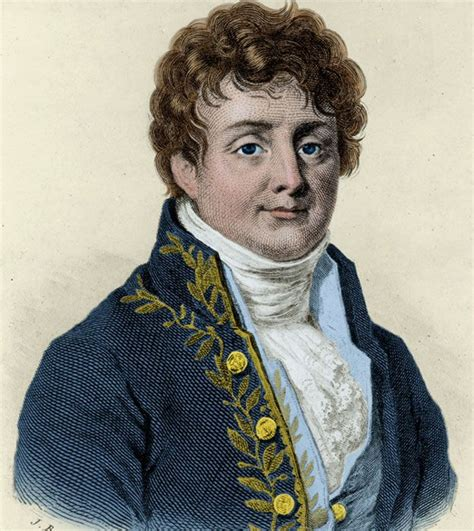
\includegraphics[height=4cm]{./fourier.jpeg}
				\hspace{1cm}
				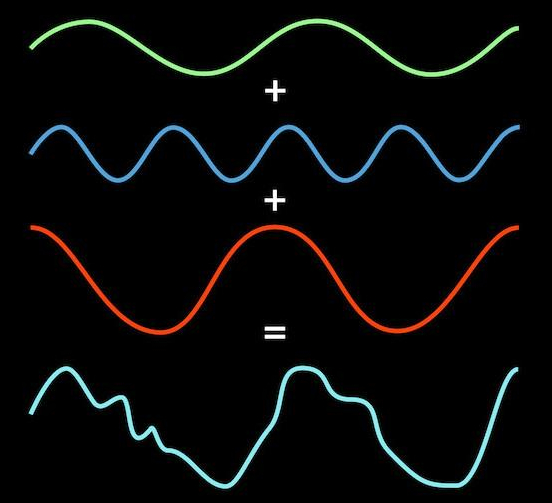
\includegraphics[height=4cm]{./fourier_dec.jpg}
			\end{figure}

		\item \texttt{JPEG2000} uses \textbf{wavelet bases}, and achieves better performance than \texttt{JPEG}.
		\item In \textbf{Homework 4}, you will use wavelets to compress/denoise images.
	\end{itemize}
\end{frame}
\appendix
\backupbegin
\begin{frame}
	\frametitle{Questions?}
\end{frame}
\backupend

\end{document}
